% begin module volumes-ex2
\begin{frame}
\begin{example}
Find the volume of the solid obtained by rotating about the $x$-axis the region under the curve $y = \sqrt{x}$ \alertNoH{23}{from $0$ to $1$}.
\begin{itemize}
\item<handout:2-|13->  The cross-sections of this solid are all circles.
\item<handout:2-|15->  The circular cross-section through the \alertNoH{15}{point $(x, 0)$} has \alertNoH{16}{radius $\sqrt{x}$}.
\item<handout:2-|17->  The area of the cross-section is \alertNoH{17,18}{$ \alertNoH{24}{A(x)} =  \fcAnswerNoH{18}{\pi \left(\sqrt{x}\right)^2 \alertNoH{24}{ = \pi x}.}$}
\item<handout:3|19->  The volume of a single approximating section is $\alertNoH{20}{ A(x)  \Delta x }$.
\item<handout:3|23->  The \alertNoH{23}{$x$ coords.} of the solid \alertNoH{23}{are between $0$ and $1$}, so its volume is
\end{itemize}
\vskip -0.15cm
\begin{columns}[c]
\column{.4\textwidth}
\begin{center}
\psset{xunit=1cm, yunit=1cm}
\begin{pspicture}(-1.8,-1.8)(1.8,1.8)
\tiny%
\renewcommand{\fcScreenStyle}{x}%
\renewcommand{\fcScreen}{[0 0 -1] 0}%
\renewcommand{\fcIterationsU}{4}%
\fcBoundingBox{-1.8}{-1.8}{1.8}{1.8}%
\only<3->{\renewcommand{\fcScreen}{[-0.05 -0.05 -1] 0}}%
\only<4->{\renewcommand{\fcScreen}{[-0.1 -0.1 -1] 0}}%
\only<5->{\renewcommand{\fcScreen}{[-0.15 -0.15 -1] 0}}%
\only<6->{\renewcommand{\fcScreen}{[-0.2 -0.2 -1] 0}}%
\only<7->{\renewcommand{\fcScreen}{[-0.25 -0.25 -1] 0}}%
\fcStartIIIdScene%
\only<3->{\fcPutIIId{[-0.1 -0.1 1.6]}{$z$}}%
\fcPutIIId{[0 1.6 ]}{$y$}%
\fcPutIIId{[1.6 0 0]}{$x$}%
\only<handout:2|14-18>{\fcSurfaceInScene[arrows=(none), linecolor=cyan, colorUV=cyan, iterationsV=5, iterationsU=1] {0.04 }{0}{2 3 div sqrt}{40 9 mul}{[2 3 div v cos u mul v sin u mul]}{}}%
\fcAxesIIIdSymmetricInScene{1.5}{1.5}{1.5}%
\only<handout:0|9>{\fcSurfaceInScene[iterationsV=3, iterationsU=3, arrows=(none), linecolor=black, linewidth=0.3]{0.01 }{0}{1}{40 3 mul}{[u u sqrt v cos mul u sqrt v sin mul]}{}%
\fcSurfaceInScene[iterationsV=3, iterationsU=1]{0.04}{ 0}{ 1}{ 40 3 mul}{[1 v cos u mul v sin u mul]}{}%
}%
\only<handout:0|10>{\fcSurfaceInScene[iterationsV=5, iterationsU=3, arrows=(none), linecolor=black, linewidth=0.3]{0.01 }{0}{1}{40 5 mul}{[u u sqrt v cos mul u sqrt v sin mul]}{}%
\fcSurfaceInScene[iterationsV=5, iterationsU=1]{0.04}{0}{1}{40 5 mul}{[1 v cos u mul v sin u mul]}{}%
}%
\only<handout:0|11>{\fcSurfaceInScene[iterationsV=7, iterationsU=3, arrows=(none), linecolor=black, linewidth=0.3]{0.04 }{0}{1}{40 7 mul}{[u u sqrt v cos mul u sqrt v sin mul]}{}%
\fcSurfaceInScene[iterationsV=7, iterationsU=1]{0.04}{0}{1}{40 7 mul}{[1 v cos u mul v sin u mul]}{}%
}%
\only<handout:1|12,13,21->{\fcSurfaceInScene[iterationsV=9, iterationsU=3, arrows=(none), linecolor=black, linewidth=0.3]{0.01 }{0}{1}{40 9 mul}{[u u sqrt v cos mul u sqrt v sin mul]}{}%
\fcSurfaceInScene[iterationsV=9, iterationsU=1]{0.04}{0}{1}{40 9 mul}{[1 v cos u mul v sin u mul]}{}%
}%
\only<handout:0|13>{\fcCurveIIIdInScene[arrows=(none), linewidth=2, linecolor=blue]{0 }{360 }{[2 3 div t cos 2 3 div sqrt 0.01 add mul t sin 0.6 sqrt 0.01 add mul]}}%
\only<2->{\fcCurveIIIdInScene[linewidth=1.5, arrows=(none), linecolor=\fcColorGraph]{0}{1}{[t t sqrt 0]}}%
\only<handout:3|19-20>{\fcSurfaceInScene[arrows=(none), linecolor=cyan, colorUV=cyan, linewidth=0.3, iterationsV=5, iterationsU=1] {0.04 }{0}{2 3 div sqrt}{40 9 mul}{[2 3 div 0.05 add v cos u mul v sin u mul]}{}%
\fcSurfaceInScene[iterationsV=9, iterationsU=1, arrows=(none), linecolor=blue, linewidth=1, colorUV=cyan, colorVU=blue]{2 3 div 0.05 sub }{0}{2 3 div 0.05 add}{360}{[u v cos 2 3 div sqrt mul v sin 2 3 div sqrt mul]}{}%
}%
\fcFinishIIIdScene[true]%
\only<handout:2|14-20>{\fcDotIIId{[2 3 div 0 0]}}%
\only<handout:2|15-20>{\fcPutIIId{[2 3 div 0.1 add -0.2 0]}{$(x,0)$}}%
\fcPutIIId{[0.5 1.2  0 ]}{$y=\sqrt{x}$}%
\only<handout:2|16-20>{\fcLineIIId[linewidth=1pt, linecolor= red]{ [2 3 div 0 0]}{[2 3 div dup sqrt 0]}}%
\uncover<handout:2|14-18>{\fcCurveIIId[linecolor=blue]{0}{360}{[2 3 div t cos 2 3 div sqrt mul t sin 2 3 div sqrt mul]}}
\uncover<handout:3|19>{\fcCurveIIId[linecolor=blue]{0}{360}{[2 3 div 0.05 add t cos 2 3 div sqrt mul t sin 2 3 div sqrt mul]}}
\only<8->{\fcCurveIIId[arrows=->, linewidth=2pt, linecolor=cyan]{-90 }{120 }{[-1.3 t cos 0.4 mul t sin 0.4 mul]}%
\fcCurveIIId[arrows=(none), linewidth=2pt, linecolor=cyan]{110 }{245 }{[-1.3 t cos 0.4 mul t sin 0.4 mul]}%
}%
\only<handout:0|23->{\fcLineIIId[linewidth=1.5pt, linecolor=red]{[0 0 0]}{[1 0 0]}%
\fcDotIIId[linecolor=red]{[0 0 0]}%
\fcDotIIId[linecolor=red]{[1 0 0]}%
}%
\end{pspicture}
%\only<handout:0| 1>{%
%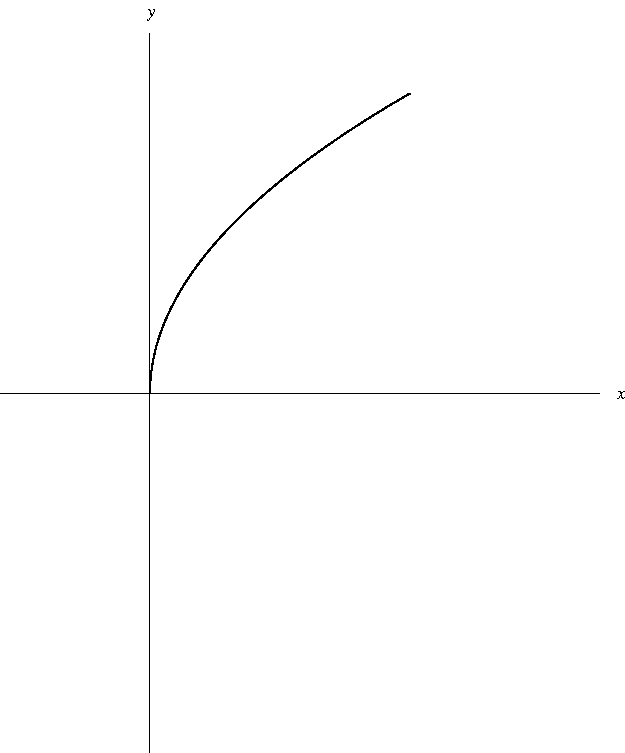
\includegraphics[height=3.5cm]{volumes/pictures/06-02-ex2a.pdf} %
%}%
%\only<handout:0| 2>{%
%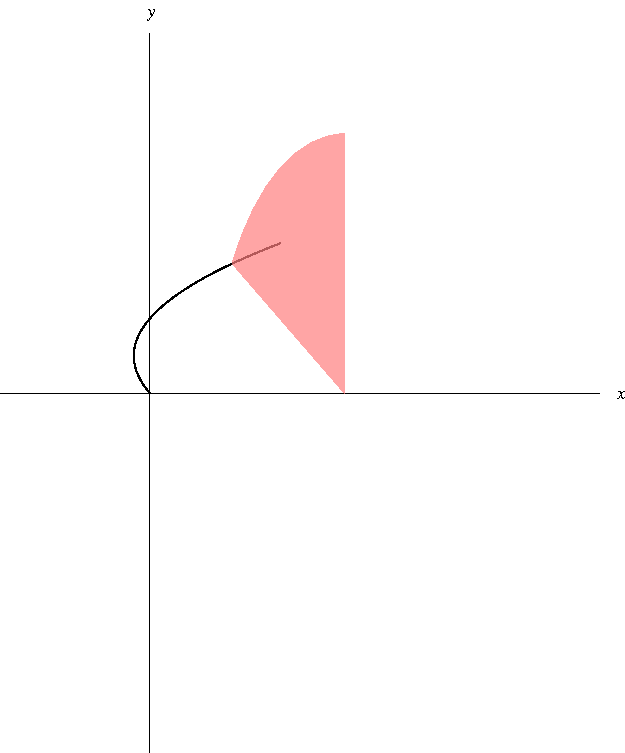
\includegraphics[height=3.5cm]{volumes/pictures/06-02-ex2b.pdf} %
%}%
%\only<handout:0| 3>{%
%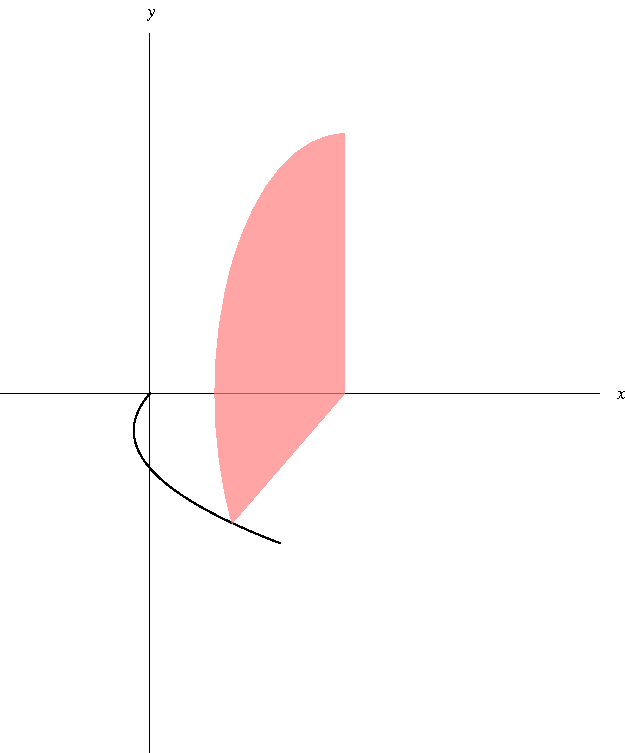
\includegraphics[height=3.5cm]{volumes/pictures/06-02-ex2c.pdf} %
%}%
%\only<handout:0| 4>{%
%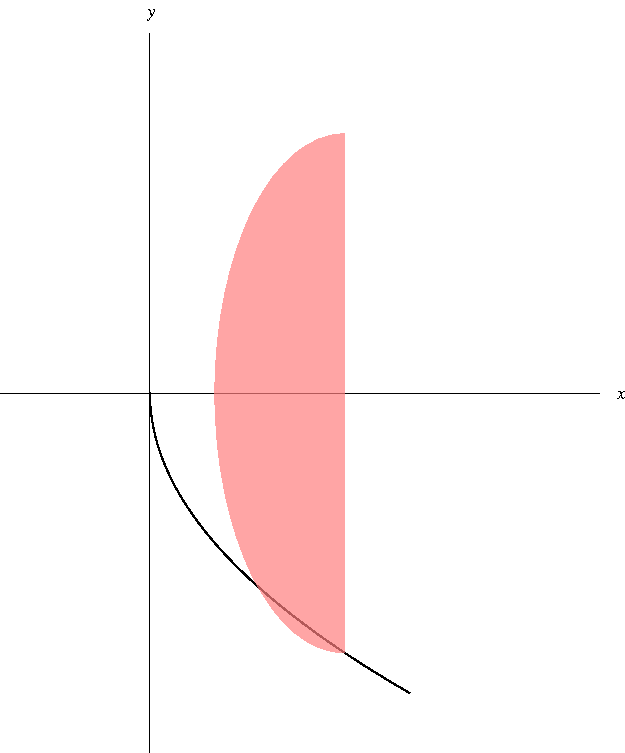
\includegraphics[height=3.5cm]{volumes/pictures/06-02-ex2d.pdf} %
%}%
%\only<handout:0| 5>{%
%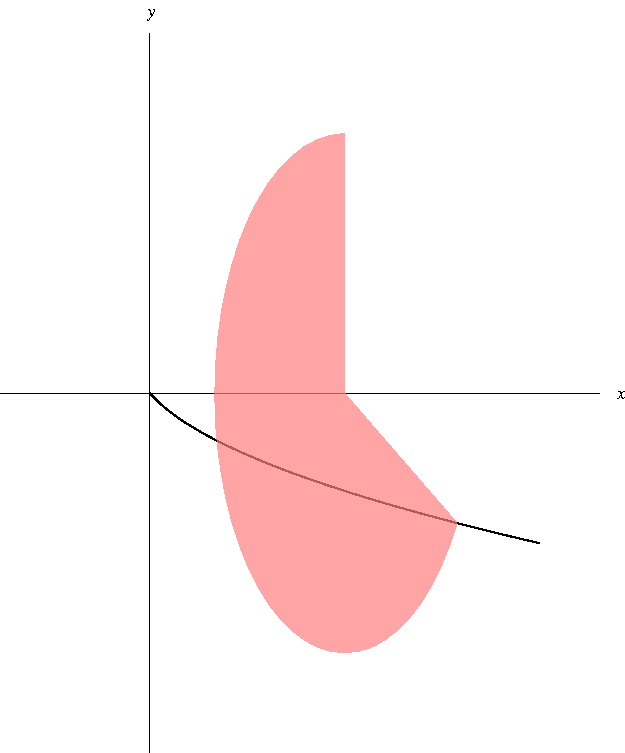
\includegraphics[height=3.5cm]{volumes/pictures/06-02-ex2e.pdf} %
%}%
%\only<handout:0| 6>{%
%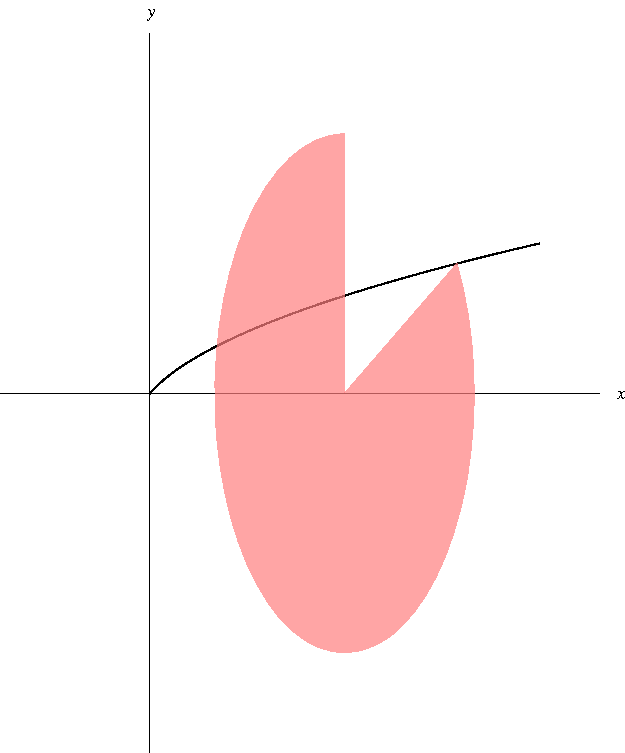
\includegraphics[height=3.5cm]{volumes/pictures/06-02-ex2f.pdf} %
%}%
%\only<7->{%
%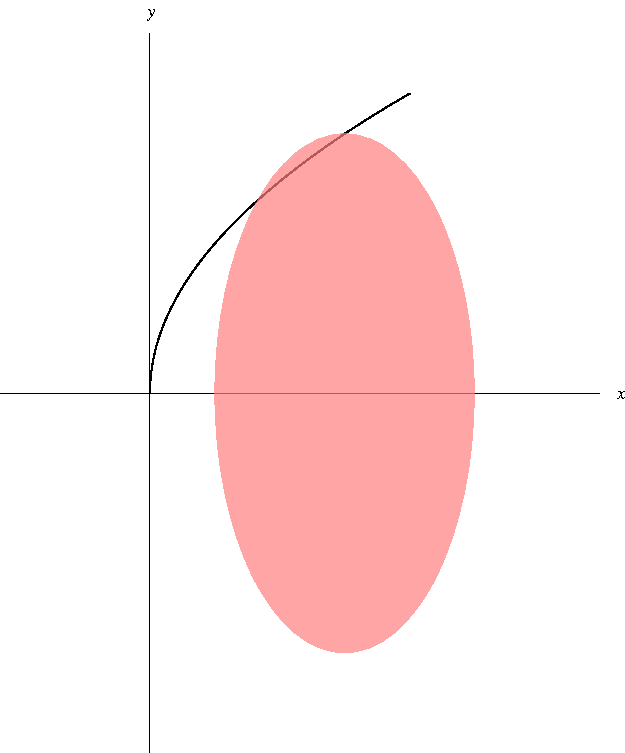
\includegraphics[height=3.5cm]{volumes/pictures/06-02-ex2g.pdf} %
%}%
\end{center}
\column{.6\textwidth}
\abovedisplayskip=0pt
\belowdisplayskip=0pt
\abovedisplayshortskip=0pt
\belowdisplayshortskip=0pt
\uncover<handout:3|1->{
\[
\begin{array}{rcl}
\uncover<20->{V & = &\displaystyle  \int_{{\fcAnswerUncover{20}{23}{0}}}^{{ \fcAnswerUncover{20}{23}{1} }} \alertNoH{20}{ \alertNoH{24}{ A(x)}  \diff x}%
\uncover<24->{ = {\alertNoH{25}{\int}}_{\!\!\!0}^1 \alertNoH{25}{\alertNoH{24}{ \pi x} \ \diff x}}%
}\\%
\uncover<25->{&  =  &\displaystyle %
\left[\alertNoH{25}{ \pi \frac{x^2}{2}} \right]_0^1%
}
\uncover<26->{ = \frac{\pi}{2}\quad .}%
\end{array}
\]
}
\end{columns}
\end{example}
\end{frame}
% end module volumes-ex2
